%-------------------------------------------------------------------------------
% yum_addsynth
%-------------------------------------------------------------------------------
%
% \file        yum_addsynth.tex
% \library     Documents
% \author      Chris Ahlstrom
% \date        2015-06-07
% \update      2016-03-07
% \version     $Revision$
% \license     $XPC_GPL_LICENSE$
%
%     Provides the ADDsynth section of yoshimi-user-manual.tex.
%
%-------------------------------------------------------------------------------

\section{ADDsynth}
\label{sec:addsynth}

   The \textsl{Yoshimi} ADDsynth (also spelled "ADsynth")
   dialog is a complex dialog for creating an
   instrument.  This is the most complex, most advanced and most
   sophisticated part of the synthesizer and allows one to edit the
   parameters that apply to all the voices of ADDsynth.

   ADDsynth, a primarily additive synthesis engine, is one of the three major
   synthesis engines available in \textsl{Yoshimi}/\textsl{ZynAddSubFX}.
   The basic concept of this engine is the summation of a collection of voices,
   each of which consists of oscillators.

   "ADDsynth" (sometimes spelled "ADsynth") or "ADnote" is a complex engine
   which makes sounds by adding a number of voices. Each one has filters,
   envelopes, LFOs, morphing, modulation, resonance, etc.
   Each voice includes a very powerful
   waveform generator with up to 128 sine/non-sine harmonics. One can use
   Fourier synthesis, or if one doesn't like it, one can use
   wave-shaping/filtering of functions. This engine includes anti-aliasing.
   Modulation includes ring modulation, phase modulation, and more.
   The modulators can have any shape.
   \cite{zyndoc}

   The sum of the voices are passed through filters and amplification to
   produce the final sound. This could lead one to think that ADDsynth is just
   a bunch of minor post-processing, and at this level much of the sound
   generation is hidden.

\begin{figure}[H]
   \centering 
   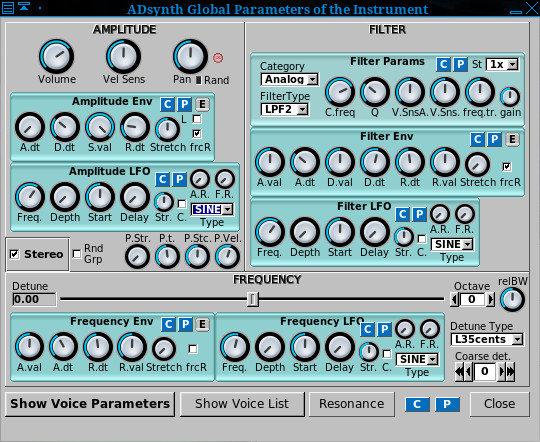
\includegraphics[scale=1.0]{bottom-panel/instrument-edit/ADD/ADDsynth-edit.jpg}
   \caption{ADDsynth Edit/Global Dialog}
   \label{fig:addsynth_edit_dialog}
\end{figure}

   The major sections of this dialog are listed:

   \begin{enumber}
      \item \textbf{AMPLITIUDE} (stock section)
      \item \textbf{FILTER} (stock section)
      \item \textbf{FREQUENCY} (stock section)
      \item \textbf{Show Voice Parameters} (section)
      \item \textbf{Show Voice List} (section)
      \item \textbf{Resonance} (stock section)
      \item \textbf{C}
      \item \textbf{P}
      \item \textbf{Close}
   \end{enumber}

   This complex dialog is best described section by section.
   Many of the sub-sections are stock sub-panels described elsewhere
   in this document.  References to those sections are included.

\subsection{ADDsynth / AMPLITUDE}
\label{subsec:addsynth_amplitude}

   \begin{enumber}
      \item \textbf{Volume}
      \item \textbf{Vel Sens}
      \item \textbf{Pan}
      \item \textbf{Rand}
      \item \textbf{Reset (panning)} (red button)
      \item \textbf{Amplitude Env}
         The Amplitude Env panel is described in detail in
         \sectionref{subsubsec:amplitude_envelope_subpanel}.
      \item \textbf{Amplitude LFO}
         The Amplitude LFO panel is described in detail in
         \sectionref{subsubsec:lfo_user_interface_panels}.
      \item \textbf{Stereo}
      \item \textbf{Rnd Grp}
      \item \textbf{P.Str.}
      \item \textbf{P.t}
      \item \textbf{P.Stc.}
      \item \textbf{P.Vel.}
   \end{enumber}

   Note the two sub-panels, mentioned above, that are described elsewhere.
   They will not be discussed in detail below.

   \setcounter{ItemCounter}{0}      % Reset the ItemCounter for this list.

   \itempar{Volume}{addsynth!volume}
   ADDsynth Volume.
   Sets the overall/relative volume of the instrument.

   Values: \texttt{1 to 127, 64*}

   \itempar{Vel Sens}{addsynth!vel sens}
   ADDsynth Velocity Sensing function.
   Velocity sensing is simply an exponental transformation from the note’s
   velocity to some parameter change.
   Observe \figureref{fig:velocity_sensing_function}.
   It shows how the velocity sensing controls affects the translation of a
   parameter over the whole range of possible note velocities.
   Turn the knob rightmost/maximum to disable this function.

   Values: \texttt{1 to 127, 64*}

\begin{figure}[H]
   \centering 
   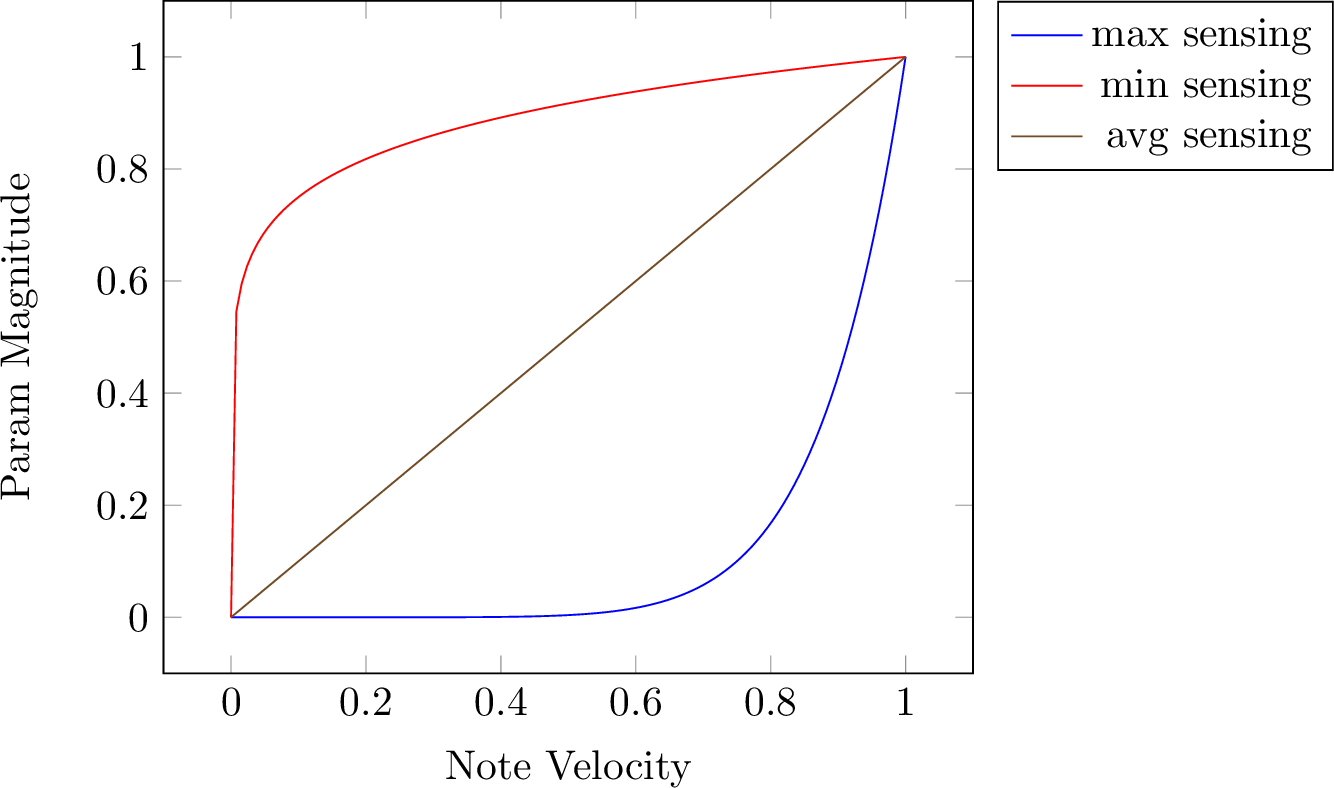
\includegraphics[scale=0.25]{zyn/velocity_sensing_function_velf.png}
   \caption{Velocity Sensing Function}
   \label{fig:velocity_sensing_function}
\end{figure}

   \itempar{Pan}{addsynth!pan}
   ADDsynth Global Panning.
   Dialing the knob to leftmost or zero gives random panning.

   Values: \texttt{0, 1 to 127, 64*}

   \itempar{Rand}{addsynth!random pan}
   ADDsynth Random Panning Indicator.
   A red fill-in color provides an indicator for the activation of random
   panning in this control.

   \itempar{Reset (panning)}{addsynth!reset pan}
   ADDsynth Reset Panning (red button).
   Clicking this red button changes the panning value to 64 (centered).

   Next, we skip the \textbf{Amplitude Env} and \textbf{Amplitude LFO}
   panels, which are described elsewhere, as noted above.

   \itempar{Stereo}{addsynth!Stereo}
   ADDsynth Stereo.
   Stereo can be enabled.
   When disabled, all the voices will also have panning disabled.

   Values: \texttt{Off, On*}

   \itempar{Rnd Grp}{addsynth!group}
   ADDsynth Random Group.
   How the harmonic amplitude is applied to voices that use the same
   oscillator.
   \index{todo!Rnd Grp}
   We need to get a more detailed explanation of what this setting means.

   Values: \texttt{Off*, On}

   \itempar{P.Str}{addsynth!punch strength}
   ADDsynth Punch Strength.
   The punch strength of a note in ADDsynth is a constant amplification to
   the output at the start of the note, with its length determined by the
   punch time and stretch and the amplitude being determined by the punch
   strength and velocity sensing. The \textbf{relBW}
   control in the frequency panel is
   effectively a multiplier for detuning all voices within an ADnote.

   Values: \texttt{0* to 127}

   \itempar{P.t}{addsynth!punch time}
   ADDsynth Punch Time (duration).
   Sets the punch effect duration (from 0.1 ms to 100 ms on an A note, 440Hz).

   Values: \texttt{0 to 127, 64*}

   \itempar{P.Stc}{addsynth!punch stretch}
   ADDsynth Punch Stretch.
   Sets the punch effect stretch according to frequency. On lower-frequency
   notes, punch stretch makes the punch effect last longer. 

   Values: \texttt{0 to 127, 64*}

   \itempar{P.Vel}{addsynth!punch vel sens}
   ADDsynth Punch Velocity Sensing.
   The higher this value, the higher the effect of velocity on the punch of
   the note.

   Values: \texttt{0 to 127, 72*}

\subsection{ADDsynth / FILTER}
\label{subsec:addsynth_filter}

   The ADDsynth FILTER block consists solely of sub-panels
   described in detail in the sections noted below.  The
   sub-panels of the FILTER section are:

   \begin{enumber}
      \item \textbf{Filter Params}
      \item \textbf{Filter Env}
      \item \textbf{Filter LFO}
   \end{enumber}

   \setcounter{ItemCounter}{0}      % Reset the ItemCounter for this list.

   \itempar{Filter Params}{addsynth!filter params}
   ADDsynth Filter Parameters.
   The Filter Params panel is described in detail in
   \sectionref{subsubsec:filter_parameters_user_interface}.

   \itempar{Filter Env}{addsynth!filter env}
   ADDsynth Filter Envelope.
   The Filter Env panel is described in detail in
   \sectionref{subsubsec:envelope_settings_for_filter}.

   \itempar{Filter LFO}{addsynth!filter lfo}
   The Filter LFO panel is described in detail in
   \sectionref{subsubsec:lfo_user_interface_panels}.

\subsection{ADDsynth / FREQUENCY}
\label{subsec:addsynth_frequency}

   \begin{enumber}
      \item \textbf{Detune}
      \item \textbf{FREQUENCY slider}
      \item \textbf{Octave}
      \item \textbf{RelBW}
      \item \textbf{Frequency Env}.
         A stock sub-panel described in
         \sectionref{subsubsec:envelope_settings_for_frequency}.
      \item \textbf{Frequency LFO}
         A stock sub-panel described in
         \sectionref{subsubsec:frequency_lfo_sub_panel}.
      \item \textbf{Detune Type}
      \item \textbf{Coarse det.}
   \end{enumber}

   \setcounter{ItemCounter}{0}      % Reset the ItemCounter for this list.

   \itempar{Detune}{addsynth!detune value}
   ADDsynth Detune Value.
   This display box shows the value of the detune as selected by the
   frequency slider described below.

\begin{figure}[H]
   \centering 
   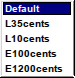
\includegraphics[scale=1.0]{bottom-panel/instrument-edit/ADD/frequency-detune-type.jpg}
   \caption{ADDsynth Frequency Detune Type}
   \label{fig:addsynth_freq_detune_type}
\end{figure}

   This value defines the number of cents that define the range of the
   \textbf{FREQUENCY} slider, that is 35 cents, 10 cents, 100 cents (one
   semitone), or 1200 cents (1 octave), below and above the main
   frequency.  The default is 35 cents.  The 1200-cents setting provides a
   whole octave of detuning in either direction.

   The "L" probably stands for "linear", and the "E" for "exponential", to
   describe how the detune slider acts.

   Values: \texttt{Default*, L35cents, L10cents, E100cents, E1200cents}

   \itempar{FREQUENCY slider}{addsynth!freq slider}
   ADDsynth Fine Detune (cents), a slider control.
   While the detune type dropdown and the octave selection provide a coarse
   selection of detune, the slider allows for a finer selection of detune,
   up to roughly one-third of a semitone.

   Values:
      \texttt{-35.00 to 35.00},
      \texttt{-10.00 to 10.00},
      \texttt{-100.00 to 100.00},
      \texttt{-1200.00 to 1200.00}

   \itempar{Octave}{addsynth!octave}
   ADDSynth Octave.
   The octave setting changes the frequency by octaves.

   Values: \texttt{-8 to 7, 0*}

   \itempar{RelBW}{addsynth!relative bw}
   ADDSynth Relative Bandwidth.
   Bandwidth: how the relative fine detune of the voice is changed.

   Values: \texttt{0 to 127, 64*}

   \itempar{Frequency Env}{addsynth!frequency env}
   ADDsynth Frequency Envelope.
   The Frequency Env panel is described in detail in
   \sectionref{subsubsec:envelope_settings_for_frequency}.

   \itempar{Frequency LFO}{addsynth!frequency lfo}
   The Frequency LFO panel is described in detail in
   \sectionref{subsubsec:lfo_user_interface_panels}

   \itempar{Detune Type}{addsynth!detune type}
   Frequency Detune Type.
   This setting provides a coarse detuning.
   We would welcome an explanation of exactly is meant by the numbers and
   the "E" versus "L" designation.

   Values: \texttt{L35cents, L10cents, E100cents, E1200cents}

   \itempar{Coarse det}{addsynth!coarse detune}
   Coarse Detune, "C.detune".
   The one-arrow buttons change the value by one.
   The two-arrow buttons change the value by ten.
   Again, we need a way to explain the interactions of the slider, the
   octave setting, the detune type, and the coarse detune settings.

   Values: \texttt{-64 to 63, 0*}

   \itempar{Show Voice Parameters}{addsynth!voice parameters}
   ADDsynth Show Voice Parameters.
   This button brings up the "voice parameters" dialog discussed in the next
   section.
   Again, this dialog is built from some stock sections and stock
   sub-panels, plus additional elements.

\subsection{ADDsynth / Voice Parameters}
\label{subsec:addsynth_voice_parameters}

   Each \textsl{Yoshimi} ADDsynth instrument consists of up to 8 voices.
   This dialog provides a way to define each of the 8 voices in great
   detail.  By default, an ADDsynth instrument consists of one voice, voice 1.

\begin{figure}[H]
   \centering 
%  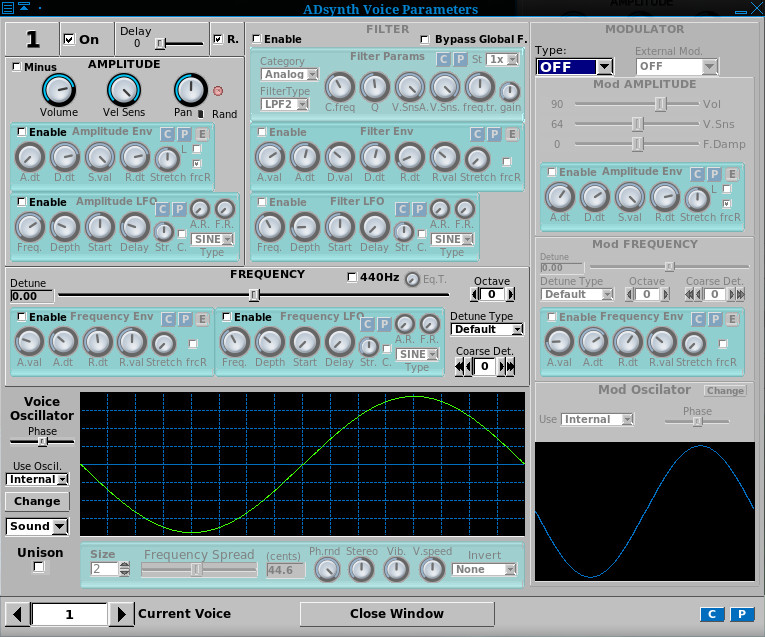
\includegraphics[scale=0.75]{bottom-panel/instrument-edit/ADD/ADDsynth-voice-parameters.jpg}
   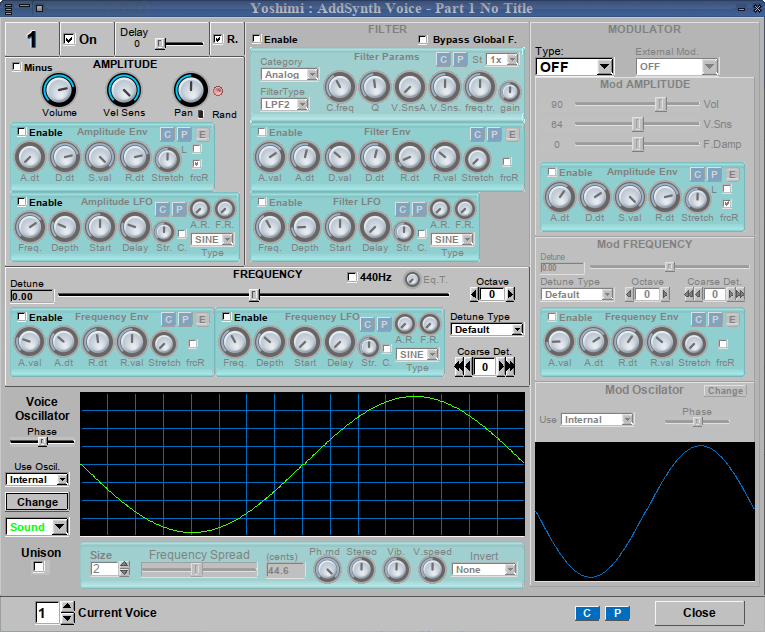
\includegraphics[scale=0.75]{1.3.9/ADDsynth-voice-parameters.png}
   \caption{ADDsynth Voice Parameters Dialog}
   \label{fig:addsynth_voice_parameters_dialog}
\end{figure}

   This dialog consists of a few extra settings, plus a number of
   stock dialog sections.  Take some time to compare
   \figureref{fig:addsynth_edit_dialog},
   which covers the overall instrument, with 
   \figureref{fig:addsynth_voice_parameters_dialog},
   which covers each of the voices.
   The stock sections in the former cover the whole instrument as one,
   while the very similar stock sections in the latter cover only the
   voice they configure.
   Obviously, the combinations of settings are essentially endless.

   Each voice can be amplitude-controlled, filter-controlled, and
   frequency-controlled.  Each voice can also be modulated by an
   internal modulator.
   Another property of the voice is that one can tell \textsl{Yoshimi}
   to modulate a given voice with any of the voices that are numbered less
   than that voice.

   \begin{enumber}
      \item \textbf{Voice Number}
      \item \textbf{On}
      \item \textbf{Delay}
      \item \textbf{R.}
      \item \textbf{AMPLITUDE} (see the stock-panel section below)
      \item \textbf{FILTER} (see the stock-panel section below)
      \item \textbf{MODULATOR} (see the stock-panel section below)
      \item \textbf{FREQUENCY} (see the stock-panel section below)
   \end{enumber}

   \setcounter{ItemCounter}{0}      % Reset the ItemCounter for this list.

   \itempar{Voice Number}{voice!number}
   ADDsynth Voice Number.
   This display element shows the voice number represented by the settings
   in this dialog.  Each \textsl{Yoshimi} part/instrument can consist of up
   to eight voices.
   The voice being worked on can be selected using the
   \textbf{Current Voice} selector.

   Values: \texttt{1* to 8}

   \itempar{On}{voice!on/off}
   ADDsynth Voice On/Off.
   Enables this voice in the part/instrument.

   Values: \texttt{Off, On}

   \itempar{Delay}{voice!delay}
   ADDsynth Voice Delay.
   \index{todo!voice delay units}
   We still need to determine what the units of the delay are.

   \textbf{Bug:}
   \index{bugs!ADDsynth voice delay tooltip}
   The tooltip for this setting says "Volume".

   Values: \texttt{0* to 127}

   \itempar{R}{voice!resonance}
   ADDsynth Voice Resonance On/Off.
   The rest of the GUI elements
   (AMPLITUDE, FILTER, MODULATOR, FREQUENCY, and Voice Oscillator)
   are more detailed, and discussed in the sections that follow.

   Values: \texttt{Off, On*}

\subsubsection{ADDsynth / Voice Parameters / AMPLITUDE}
\label{subsubsec:addsynth_voice_parameters_amplitude}

   This section of the voice parameters dialog also includes a couple of
   stock sub-panels that have an additional "Enable" control.

   \begin{enumber}
      \item \textbf{Minus}
      \item \textbf{Volume}
      \item \textbf{Vel Sens}
      \item \textbf{Pan}
      \item \textbf{Pan randomness indicator}
      \item \textbf{Pan reset} (red button)
      \item \textbf{Amplitude Env, Stock + Enable}
      \item \textbf{Amplitude LFO, Stock + Enable}
   \end{enumber}

   \setcounter{ItemCounter}{0}      % Reset the ItemCounter for this list.

   \itempar{Minus}{voice par amp!invert vol control}
   ADDsynth Amplitude Minus.
   This setting enables the inversion of the volume control action.
   It enables negative values for the volume control of the voice.

   Values: \texttt{Off*, On}

   \itempar{Volume}{voice par amp!volume}
   ADDsynth Voice Volume.
   Sets the (relative) volume of this voice in the part/instrument.

   Values: \texttt{0 to 127, 90?}

   \itempar{Vel Sens}{voice par amp!vel sens}
   ADDsynth Voice velocity-sensing function; setting to rightmost/max
   disables this function.

   Values: \texttt{0 to 127*}

   \itempar{Pan}{voice par amp!pan}
   ADDsynth Voice panning; setting to leftmost/0 gives random panning.

   Values: \texttt{0 to 127, 64*}

   \itempar{Pan randomness indicator}{voice par amp!random pan}
   ADDsynth Voice random panning On/Off.
   Fills in red to indicate that random panning is in force.

   \itempar{Pan reset (red button)}{voice par amp!center pan}
   ADDsynth Center Panning.
   Clicking this small red button resets the panning to center.

   \itempar{Amplitude Env, Stock + Enable}{voice par amp!amp env}
   ADDsynth Amplitude Envelope Sub-panel.
   See \sectionref{subsubsec:amplitude_envelope_subpanel}.
   Additionally, the \textbf{Enable} checkbox allows the enabling of this
   component.

   \itempar{Amplitude LFO, Stock + Enable}{voice par amp!amp lfo}
   ADDsynth Amplitude LFO Sub-panel.
   See \sectionref{subsubsec:lfo_user_interface_panels}.
   Additionally, the \textbf{Enable} checkbox allows the enabling of this
   component.

\subsubsection{ADDsynth / Voice Parameters / FILTER}
\label{subsubsec:addsynth_voice_parameters_filter}

   This section of the voice parameters dialog also includes a couple of
   stock sub-panels that have an additional "Enable" control.

   \begin{enumber}
      \item \textbf{Enable}
      \item \textbf{Bypass Global F.}
      \item \textbf{Filter Params, Stock}
      \item \textbf{Filter Env, Stock + Enable}
      \item \textbf{Filter LFO, Stock + Enable}
   \end{enumber}

   \setcounter{ItemCounter}{0}      % Reset the ItemCounter for this list.

   \itempar{Enable}{voice par filter!enable}
   ADDsynth Voice Enable Filter.
   This value enables the whole FILTER dialog section.

   Values: \texttt{Off*, On}

   \itempar{Bypass Global F}{voice par filter!bypass}
   ADDsynth Voice Bypass Global Filter.
   The voice signal bypasses the global filter.

   Values: \texttt{Off*, On}

   \index{todo!global filter}
   We need to make sure there is a discussion of the global filter.

   \itempar{Filter Params, Stock}{voice par filter!parameters}
   See \sectionref{subsubsec:filter_parameters_user_interface}.

   \itempar{Filter Env, Stock + Enable}{voice par filter!env}
   See \sectionref{subsubsec:envelope_settings_for_filter}.

   \itempar{Filter LFO, Stock + Enable}{voice par filter!lfo}
   See \sectionref{subsubsec:filter_lfo_sub_panel}.

\subsubsection{ADDsynth / Voice Parameters / MODULATOR}
\label{subsubsec:addsynth_voice_parameters_modulator}

   \begin{enumber}
      \item \textbf{Type:}
      \item \textbf{External Mod.}
      \item \textbf{Mod AMPLITUDE}
      \item \textbf{Mod FREQUENCY}
      \item \textbf{Mod Oscillator}
   \end{enumber}

   \setcounter{ItemCounter}{0}      % Reset the ItemCounter for this list.

   \itempar{Type:}{modulator!type}
   ADDsynth Modulator Type.

\begin{figure}[H]
   \centering 
   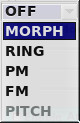
\includegraphics[scale=0.75]{bottom-panel/instrument-edit/ADD/modulator-type.jpg}
   \caption{Voice Modulator Type}
   \label{fig:voice_modulator_type}
\end{figure}

   \begin{enumber}
      \item \textbf{OFF}.
         This setting turns off the modulator.
      \item \textbf{MORPH}
         \index{MORPH}
         \index{morph modulator}
         \index{modulator!morph}
         The morph modulator works by combining the output of two oscillators
         into one, with the amplitude envelope translating between one waveform
         and the other.
      \item \textbf{RING}
         \index{RING}
         \index{ring modulator}
         \index{modulator!ring}
         The ring modulator is useful for making bell-like sounds and some
         weird effects.  The ring modulator works by multiplying two
         waveforms together, producing a signal that possesses the sum and
         difference of the frequencies present in the waveforms.  The
         ins-and-outs of the ring modulator are explained in detail in
         \paragraphref{paragraph:tips_using_the_ring_modulator}.
      \item \textbf{PM}
         \index{PM}
         \index{pulse modulator}
         \index{modulator!pulse}
         The PM (pulse modulation) modulator works by using a modulator
         envelope to change the pulse width of a pulse waveform.
         Generally, set \textbf{F.Damp} to zero, so that the modulation amount
         doesn't depend on the note number.
      \item \textbf{FM}
         \index{FM}
         \index{frequency modulator}
         \index{modulator!frequency}
         The (frequency modulation) morph modulator works by modulator the
         frequency.  Examples can be heard in the "Ethereal" and "Steel Wire"
         instruments.
      \item \textbf{PITCH}
         \index{PITCH}
         \index{pitch modulator}
         \index{modulator!pitch}
         The pitch modulator works by...
         we're not sure... is this pitch shifting?
   \end{enumber}

   Values: \texttt{OFF, MORPH, RING, PM, FM, PITCH}

   \itempar{External Mod}{modulator!external}

   \textbf{External Oscillator}.
   \index{oscillator!external}
   This feature allows one of the voices (of the up to 8 allowed in a single
   ADDsynth instrument) to be used as a modulator or external oscillator for
   another voice in the instrument.
   This option specifies to use the oscillator of another voice, or
   -1 for the \textsl{internal} oscillator.
   \index{oscillator!internal}

   The parameters must be lower than the voice index; one cannot use the
   oscillator from a voice with a bigger index (e.g. one can't use the
   oscillator of voice 8 for voice 4). This is very useful because, if
   one uses many voices with the same oscillator settings, one can use only
   one oscillator and select other voices to use this, and if one changes a
   parameter of this oscillator, all voices using this oscillator will be
   affected.

   \textbf{External Modulator}.
   \index{modulator!external}
   Use another voice as a modulator instead of the modulator of the internal
   voice. One can make a modulation "stack". The modulator of the voice is
   disabled. 

   \textbf{External}.
   Uses the oscillator as the modulator of another voice. It
   behaves like \textbf{Ext. Oscil}, except that it works on the
   \textsl{modulator}. Please
   notice the difference between this parameter and \textbf{Ext. Mod}. 
   See below.

   Values: \texttt{OFF*, Other voice numbers?}

   \itempar{Mod AMPLITUDE}{modulator!amplitude}
   Modulator Amplitude.

   \begin{enumber}
      \item \textbf{Vol}
         Volume.
         Values: \texttt{0 to 127, 90*}
      \item \textbf{V.Sns}
         Velocity Sensing Function; set to rightmost/max to disable.
         Values: \texttt{0 to 127, 64*}
      \item \textbf{F.Damp}
         Modulator Damp at higher frequency.
         How the modulator intensity is lowered according to lower/higher
         note frequencies. 
         Values: \texttt{0 to 127, 90*}
      \item \textbf{Amplitude Env, Stock + Enable}
         See \sectionref{subsubsec:amplitude_envelope_subpanel}.
   \end{enumber}

   \itempar{Mod FREQUENCY}{modulator!frequency}
   Modulator Frequency.

   \begin{enumber}
      \item \textbf{Detune slider}
         Fine Detune (cents).
         Values: \texttt{-35.00 to 35.00, 0*}
      \item \textbf{Detune Type}
         Fine Detune (cents).
         Values: \texttt{L35cents, L10cents, E100cents, E1200cents}
         See \figureref{fig:addsynth_freq_detune_type}.
      \item \textbf{Octave}
         Octave.
         Values: \texttt{-8 to 7, 0*}
      \item \textbf{Coarse Det.}
         Coarse Detune.
         Values: \texttt{-64 to 63, 0*}
      \item \textbf{Filter Env, Stock + Enable}
         See \sectionref{subsubsec:envelope_settings_for_filter}.
   \end{enumber}

   \itempar{Mod Oscillator}{modulator!oscillator}
   Modulator Oscillator.

   \textbf{Bug:}
   \index{bugs!mod oscillator name mispelled}
   The word "oscillator" is mispelled in the application.

   \begin{enumber}
      \item \textbf{Change}
         ADDsynth Oscillator Editor.
      \item \textbf{Use}
         Oscillator to Use.
         See the paragraph below.
         Values: \texttt{Internal*, Other oscillators?}
      \item \textbf{Phase}
         Oscillator Phase.
         Values: \texttt{0 to 360 (0 to 2PI)}
      \item \textbf{Waveform graph}
         Waveform graph.
   \end{enumber}

   As far as we can tell, one has the choice between \textbf{Internal},
   which in this case means a completely independent modulator oscillator
   per voice (extra change button), or \textbf{External}, which refers to
   the modulation oscillators one has already defined for the voices with a
   lower index.
   This means one can make one modulation oscillator for voice 1, and reuse it
   in voices 2 and 3.  This is the same system used for the normal
   oscillators.

\paragraph{Tip: Using the Ring Modulator}
\label{paragraph:tips_using_the_ring_modulator}
\index{tips!ring modulator}
\index{tips!internal modulator}

   This section is derived from one of the short text files in the
   \textsl{Yoshimi} source-code bundle (\cite{yoshimi} or \cite{yoshimi2}).
   It notes that "Some people have
   been confused about how to use an 'external' Mod Oscillator", and
   provides usage notes that we will elaborate on here.  Here is the way to
   use the ring modulator:

   \begin{enumber}
      \item Open the ADDsynth editing window.  Then open
         \textbf{Show Voice Parameters}.
      \item For \textbf{Type}, select the \textbf{RING} value.  This
         selection will activate the \textbf{Mod Oscillator}.
      \item In the \textbf{Mod Oscillator}, click on \textbf{Change} to open
         the \textbf{ADDsynth Oscillator Editor}.
      \item Set the wave-shape to \textbf{Triangle}.
      \item Switch to voice number 2 and enable it.
      \item Again, for \textbf{Type}, select the \textbf{RING} value.
         However, feel free to select one of the other modulators, if one
         wishes.
      \item One can now use \textbf{Internal} for voice 2, or select
         \textbf{ext.m} 1, to use the first voice as in internal modulator.
      \item Change the internal voice to, for example, \textbf{Square}.
      \item Do the same setup for voice 3.
         One will find that one can use its \textbf{Internal} or
         either of the two previous ones.
   \end{enumber}

   Now the joker in the pack is that one can disable both the previous
   voices but \textsl{still} use their Mod Oscillators.

   In a newsgroup (\cite{ringmodulator}, the following note is found.

   \begin{quotation}
      Say I want the A tone ring-modulated by 880Hz. A is 440 Hz, the ring
      modulation setting lets me choose the modulation frequency relative
      to the frequency of the tone. So I choose octave 1 and let the
      detune at zero. If I move the detune, it'll shift the modulation
      frequency a bit, which will make a disharmonic effect.

      Wet/dry setting is controlled by volume in "modulation amplitude".
      The modulation frequency can further be multiplied or several
      modulations can be simulated by changing the oscillator waveform.

      One huge letdown is that it is only available for Adsynth. PadSynth
      does not seem to have ring modulation option, so the coolest sounds
      stay out of question for massive lead tones. :-(
   \end{quotation}

   We have provided a more useful "tutorial" on using the ring modulator in the
   \cite{cookbook} document.

\subsubsection{ADDsynth / Voice Parameters / FREQUENCY}
\label{subsubsec:addsynth_voice_parameters_frequency}

   This frequency section is almost a stock part.
   It is similar to the ADDsynth Edit's \textbf{FREQUENCY} section.

   \begin{enumber}
      \item \textbf{Detune}
      \item \textbf{FREQUENCY slider}
      \item \textbf{440Hz}          % addition to stock
      \item \textbf{Eq.T}          % addition to stock
      \item \textbf{Octave}
      \item \textbf{Detune Type}
      \item \textbf{Coarse det}
      \item \textbf{Frequency Env, Stock + Enable}
      \item \textbf{Frequency LFO, Stock + Enable}
      \item \textbf{Voice Oscillator}
   \end{enumber}

   \setcounter{ItemCounter}{0}      % Reset the ItemCounter for this list.

   \itempar{Detune}{voice parameters!detune}
   Voice Parameters Detune.
   Shows the value selected by the frequency slider.

   \itempar{FREQUENCY slider}{voice parameters!freq slider}
   Frequency Slider.
   Provides fine detune, in cents.
   Note that 35 cents is roughly one-third of a semitone.

   Values: \texttt{-35.00 to 35.00, 0*}

   \itempar{440Hz}{voice parameters!440 hz}
   440 Hz Selection.
   Fixes the voice base frequency to 440 Hz.
   One can adjust this with the detune settings.
   No matter what key is played on the keyboard, this voice will emit only
   440 Hz.  This is useful for defining a constant frequency to use as a
   modulator for the other voices in the part.
   For example, one can define voice 1 to be a tone, then
   define voice 2 to be 440 Hz.  The two voices will mix, but only voice 1
   will change frequencies as different keys are played.

   Values: \texttt{Off*, On}

   \itempar{Eq.T}{voice parameters!eq type}
   Equal Temperament?
   This item is enabled only if the \textbf{440Hz} check-box is enabled.
   It determines how the frequency varies according to the 
   keyboard.  If set to its leftmost (0) value, then the frequency is fixed.

   Values: \texttt{0 to 127?}

   \itempar{Octave}{voice parameters!octave}
   Voice Parameters Octave.

   Values: \texttt{-8 to 7, 0*}

% Where did I get this setting?  An older version of the dialog?
%
%  \itempar{RelBW}{voice parameters!relbw}
%  Relative bandwidth.

   \itempar{Detune Type}{voice parameters!fine detune}
   Detune Type.

\begin{figure}[H]
   \centering 
   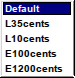
\includegraphics[scale=1.0]{bottom-panel/instrument-edit/ADD/frequency-detune-type.jpg}
   \caption{Frequency Detune Type}
   \label{fig:frequency_detune_tYpe}
\end{figure}

   Values: \texttt{Default*, L35cents, L10cents, E100cents, E1200cents}

   \itempar{Coarse det}{voice parameters!coarse detune}
   Coarse Detune.
   Is this setting in units of semitones?
   \index{todo!coarse detune units}

   Values: \texttt{-64 to 63, 0*}

   \itempar{Frequency Env, Stock + Enable}{voice parameters!freq env}
   Frequency Envelope.
   See \sectionref{subsubsec:envelope_settings_for_frequency}.

   \itempar{Frequency LFO, Stock + Enable}{voice parameters!freq lfo}
   Frequency LFO.
   See \sectionref{subsubsec:frequency_lfo_sub_panel}.

   \itempar{Voice Oscillator}{voice parameters!oscillator}
   Voice Parameters Oscillator.
   See the next section.

\subsubsection{ADDsynth / Voice Parameters / Voice Oscillator}
\label{subsubsec:addsynth_voice_parameters_oscillator}

   The ADDsynth Voice Oscillator panel is tucked in the lower left side of the
   ADDSynth Voice Parameters editor.

   \begin{enumber}
      \item \textbf{Phase}
      \item \textbf{Use}
      \item \textbf{Waveform graph}
      \item \textbf{Change}
      \item \textbf{Sound}
      \item \textbf{Unison}
      \item \textbf{Current Voice}
      \item \textbf{C}
      \item \textbf{P}
      \item \textbf{Close Window}
   \end{enumber}

   \setcounter{ItemCounter}{0}      % Reset the ItemCounter for this list.

   \itempar{Phase}{voice oscillator!phase}
   Voice Oscillator Phase.

   Values: \texttt{0 to 360 (0 to 2*pi)}

   \itempar{Use Oscil}{voice oscillator!use}
   Use Oscillator.
   If the \textbf{Current Voice} is set to a value greater than 1, meaning
   that one is editing additional voices, then this dropdown item also
   includes the values of all oscillators less then this one, marked as
   "External".  For example, if one is currently editing current voice 3,
   then the dropdown list includes \textbf{Internal}, \textbf{Ext. 1}, and
   \textbf{Ext. 2}.

   Values: \texttt{Internal*, Other oscillators}

   \itempar{Waveform graph}{voice oscillator!waveform}
   Waveform Graph.
   Shows a period of the currently configured oscillator.

   \itempar{Change}{voice oscillator!Change}
   ADDSynth Voice Oscillator Change.
   This button brings up the ADDsynth Oscillator Editor dialog.
   This dialog is described elsewhere.

   \itempar{Sound}{voice oscillator!sound}
   ADDSynth Oscillator Type (sound/noise).
   Sound/Noise choice.
   Select the mode of the oscillator (sound versus white noise).

\begin{figure}[H]
   \centering 
   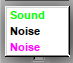
\includegraphics[scale=1.0]{1.3.9/voice-oscillator-sound-dropdown.png}
   \caption{Voice Oscillator Choices}
   \label{fig:voice_oscillator_choices}
\end{figure}

   Values: \texttt{Sound*, Noise (white), Noise (pink)}

   If white \textbf{Noise} is selected, then the waveform graph simply announces
   "White Noise".  Also, the \textbf{Unison} control is
   disabled.

\begin{figure}[H]
   \centering 
   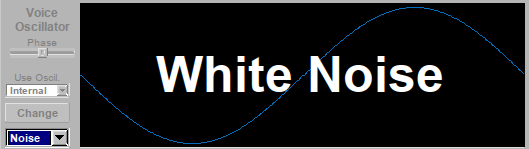
\includegraphics[scale=0.75]{1.3.9/white_noise_banner.png}
   \caption{White Noise in ADDSynth Voice}
   \label{fig:voice_oscillator_white_noise}
\end{figure}

   If white \textbf{Noise} is selected, then the waveform graph simply announces
   "Pink Noise".  Also, the \textbf{Unison} control is
   disabled.

\begin{figure}[H]
   \centering 
   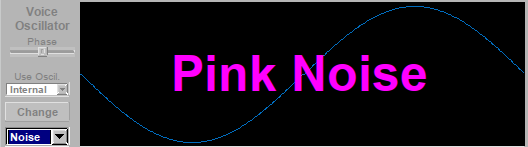
\includegraphics[scale=0.75]{1.3.9/pink_noise_banner.png}
   \caption{Pink Noise in ADDSynth Voice}
   \label{fig:voice_oscillator_pink_noise}
\end{figure}

   \itempar{Unison}{voice oscillator!Unison}
   Unison is useful in creating the chorus like sound of many simultaneous
   oscillators.

   Values: \texttt{Off*, On}

   Enabling this item causes the Unison-related items to become
   enabled (they are discussed next, starting with \textbf{Size}
   and \textbf{Frequency Spread}.

   \begin{enumber}
      \item \textbf{Size}
      \item \textbf{Frequency Spread}
      \item \textbf{Ph.rnd}
      \item \textbf{Stereo}
      \item \textbf{Vibrato}
      \item \textbf{V.speed}
      \item \textbf{Invert}
   \end{enumber}

   \setcounter{ItemCounter}{0}      % Reset the ItemCounter for this list.

   \itempar{Unison Size}{unison!size}
   Sets the number of unison sub-voices.

   Values: \texttt{2* to 50}

   \itempar{Unison Frequency Spread}{unison!freq spread}
   Frequency spread of the unison (cents).

   Values: \texttt{0 to 200, 44.6*}

   \itempar{Phase Randomness}{unison!Ph.rnd}
   Unison Phase Randomness.

   Values: \texttt{0 to 127*}

   \itempar{Stereo Spread}{unison!Stereo}
   Unison Stereo Spread.

   Values: \texttt{0 to 127, 64*}

   \itempar{Unison Vibrato}{unison!Vibrato}
   Unison Vibrato.

   Values: \texttt{0 to 127, 64*}

   \itempar{Vibrato Speed}{unison!V.speed}
   Unison Vibrato Average Speed.

   Values: \texttt{0 to 127, 64*}

   \itempar{Phase Invert}{unison!Invert}
   Unison Phase Invert.
   Values: \texttt{None*, Random, 50\%, 33\%, 25\%, 20\%}

\begin{figure}[H]
   \centering 
   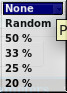
\includegraphics[scale=1.0]{bottom-panel/instrument-edit/ADD/voice-oscillator-phase-invert-dropdown.jpg}
   \caption{Unison Phase Invert Dropdown}
   \label{fig:phase_invert_dropdown}
\end{figure}

   Finally, at the bottom of the ADDsynth Voice Part dialog, we find the
   last few controls.

   \setcounter{ItemCounter}{0}      % Reset the ItemCounter for this list.

   \itempar{Current Voice}{voice oscillator!current voice}
   Current Voice.

   Values: \texttt{1* to 8}

   \itempar{C}{voice oscillator!copy}
   Copy D note parameters ("DnoteParameters").

   \itempar{P}{voice oscillator!paste}
   Paste D note parameters ("DnoteParameters").

   \itempar{Close Window}{voice oscillator!close}
   Close.

\subsection{ADDsynth / Voice List}
\label{subsec:addsynth_voice_list}

   The ADDsynth Voices List shows a summary of voices 1 to 8, and allows
   some overall control of them, almost like a simple mixer.
   It is brought on-screen via the \textbf{Show Voice List} button
   of the ADDsynth global part editor.

\begin{figure}[H]
   \centering 
   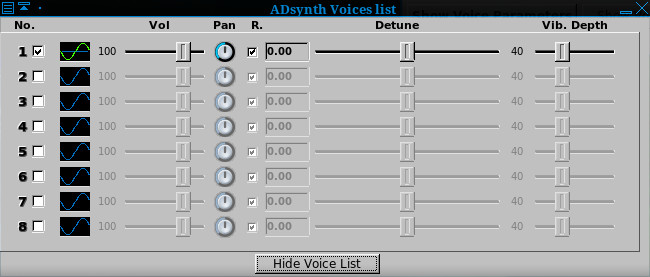
\includegraphics[scale=0.75]{bottom-panel/instrument-edit/ADD/ADDsynth-voices-list.jpg}
   \caption{ADDsynth Voices List}
   \label{fig:addsynth_voices_list}
\end{figure}

   \begin{enumber}
      \item \textbf{No. (1 to 8)}
      \item \textbf{Waveform}
      \item \textbf{Vol}
      \item \textbf{Pan}
      \item \textbf{R.}
      \item \textbf{Detune}
      \item \textbf{Vib. Depth}
      \item \textbf{Hide Voice List}
   \end{enumber}

   \setcounter{ItemCounter}{0}      % Reset the ItemCounter for this list.

   \itempar{No. (1 to 8)}{voice list!number}
   Voice List Number.
   This check-box enables or disables a given voice in the current part.

   Values: \texttt{Off, On}

   \itempar{Waveform Icon}{voice list!waveform icon}
   Waveform Icon.
   The waveform icon shows a rough rendering of the actual shape of the
   voice waveform, or the letter \textbf{N} is the voice is constructed from
   white noise.  Note that this picture isn't updated, if the voice is
   edited, until the voice list is closed and reopened.

   \itempar{Vol}{voice list!volume}
   Voice Volume.
   This slider controls the relative volume of a given voice in the current
   part.

   Values: \texttt{0 to 127, 100*}

   \itempar{Pan}{voice list!panning}
   Voice Panning (0/leftmost is Random).
   This slider controls the panning of a given voice in the current part.

   Values: \texttt{0 to 127, 64*}

   \itempar{R}{voice list!resonance}
   Resonance On/Off.
   Enable/disable the resonance effect of a voice.
   Note that the resonance is configured in by the Resonance dialog brought
   up by the \textbf{Resonance} button at the bottom of the ADDsynth main
   dialog.  The resonance dialog has its own Enable button, as well.
   These seem to be independent settings.

   Values: \texttt{Off, On*}

   \itempar{Detune Value}{voice list!detune value}
   This read-only text-box shows the current value of detune as selected by
   its slider.

   \itempar{Detune}{voice list!detune}
   Fine Detune (cents).

   Values: \texttt{-35 to 35, 0*}

   \itempar{Vib. Depth}{voice list!vibrato depth}
   Frequency LFO Amount/Depth.
   This setting can be very useful because, with the detune settings, one can
   create very good sounding instruments. 

   Values: \texttt{0 to 127, 40*}

   \itempar{Hide Voice List}{voice list!hide}
   Hide Voice List.  A Close button, really, and that is what it is in the
   latest version of \textsl{Yoshimi}.

\subsection{ADDsynth / Oscillator}
\label{subsec:addsynth_oscillator}

   Pressing the ambiguously-named \textbf{Change} button in the ADDsynth
   voice-editor dialog brings up a very complex dialog for modifying the
   harmonics of the voice.

\begin{figure}[H]
   \centering 
   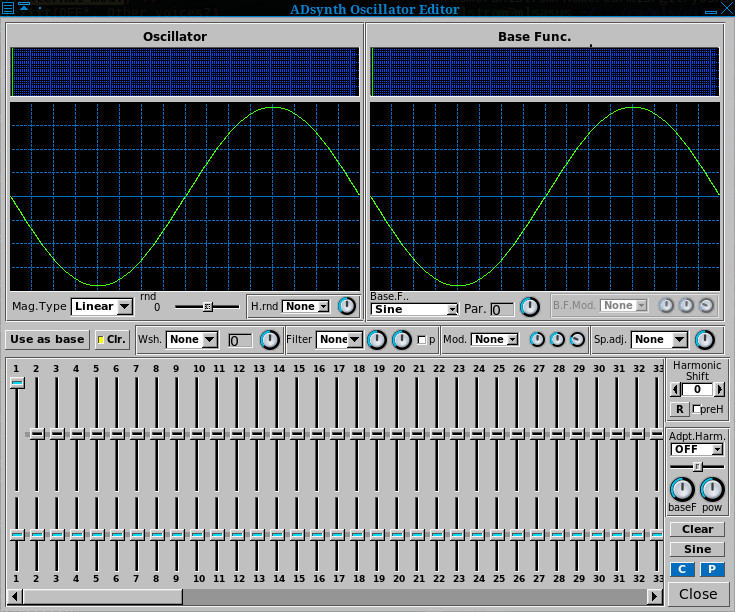
\includegraphics[scale=0.75]{bottom-panel/instrument-edit/ADD/ADDsynth-oscillator-editor.jpg}
   \caption{ADDsynth Oscillator Editor}
   \label{fig:addsynth_oscillator_editor}
\end{figure}

   This item is nearly identical to the PADsynth harmonic editor depicted in
   \figureref{fig:padsynth_harmonic_content_editor},
   except for the items noted below.
   Obviously, it is a topic unto itself!

   \begin{enumber}
      \item \textbf{Oscillator Spectrum Graph}
      \item \textbf{Oscillator Waveform Graph}
      \item \textbf{Mag.Type}
      \item \textbf{rnd} (ADDsynth Oscillator Editor only)
      \item \textbf{H.rnd} (ADDsynth Oscillator Editor only)
      \item \textbf{H.rnd knob} (ADDsynth Oscillator Editor only)
   \end{enumber}

   \setcounter{ItemCounter}{0}      % Reset the ItemCounter for this list.

   \itempar{Oscillator Spectrum Graph}{addsynth!oscillator graph}
   Oscillator Spectrum Graph.
   This graph shows the spectrum of the oscillator as a series of vertical
   lines, a kind of frequency histogram.

   \itempar{Oscillator Waveform Graph}{addsynth!waveform graph}
   Oscillator Waveform Graph.
   This graph shows the temporal waveform  of the oscillator.

   \itempar{Mag.Type}{addsynth!mag type}
   Oscillator Magnitude Type.
   Sets how the magnitudes from the user interface behave.  See the values
   below.

   \itempar{rnd}{addsynth!rnd}
   rnd. Sets the randomness of the oscillator output. There are 2 types of
   randomness provided.  The first type of randomness is
   \textsl{group randomness},
   \index{group randomness}
   \index{randomness!group}
   where the oscillator starts at random positions within the waveform,
   and the second type of randomness is
   \textsl{phase randomness},
   \index{phase randomness}
   \index{randomness!phase}
   which is settable from -64 (the maximum) to -1 (the minimum),
   the oscillator is phase distorted,
   and each harmonic is from 1 (the maximum) to 63 (the minimum).
   A setting of zero (0) is no randomness.
   One can use this parameter to make warm sounds like
   analogue synthesizers.

   \itempar{H.rnd}{addsynth!H.rnd}
   Harmonic Amplitude Randomness.
   Adjusts how the randomness is employed.
   Not sure how this works, so, for now, experiment!

\begin{figure}[H]
   \centering 
   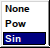
\includegraphics[scale=1.0]{bottom-panel/instrument-edit/ADD/ADDsynth-hrnd.png}
   \caption{ADDsynth Oscillator Harmonic Randomness Selections}
   \label{fig:addsynth_hrnd}
\end{figure}

   Values: \texttt{None, Pow, and Sin}

   \itempar{H.rnd knob}{addsynth!H.rnd knob}
   Harmonic Amplitude Randomness Knob.
   This knob provides the oscillator's spectrum-adjust parameter.

   Values: \texttt{0 to 127, 64*}

\subsection{ADDsynth / Resonance}
\label{subsec:addsynth_resonance}

   This dialog, shared in common with the PADsynth editor, is a stock
   user-interface element described in
   \sectionref{subsec:stock_resonance_settings}.

%-------------------------------------------------------------------------------
% vim: ts=3 sw=3 et ft=tex
%-------------------------------------------------------------------------------
